\chapter{OFDM in Gnu Radio}
\label{cha:789}
La prima parte del lavoro svolto è consistita nell'implementazione di OFDM nell'ambiente GnuRadio. Il funzionamento di OFDM necessita di vari meccanismi complessi come l'assegnazione di informazioni alle sottoportanti, le correzioni in frequenza, l'equalizzazione e la correzione d'errore come precedentemente spiegato nella parte teorica. Lo svolgimento di queste operazioni sono rese possibili dalla presenza sia di blocchi generici utili ad esempio per la correzione d'errore che di blocchi disponibili specificamente per l'implementazione di OFDM. Per una comunicazione standard OFDM in Gnuradio non è necessaria la scrittura di algoritmi eventualmente importabili sotto forma di blocchi personalizzati, il lavoro consiste nel collegamento e nella configurazione dei parametri al fine di farli comunicare nella maniera corretta.
La comunicazione è divisa in due parti, una per la trasmissione che ha il compito di generare campioni per il driver dell'usrp-sdr ed una per la ricezione che partendo dai campionamenti effettuati dall'rtl-sdr decodifica le informazioni. Di seguito verranno documentate parte per parte tutte le fasi necessarie.

 \section{Trasmettitore}
 La trasmissione è composta da quattro sezioni principali connesse fra loro.
 \begin{itemize}
 	\item \subsection{Formazione pacchetti dal flusso in ingresso}
 	\begin{figure}[h]
 		\centering
 		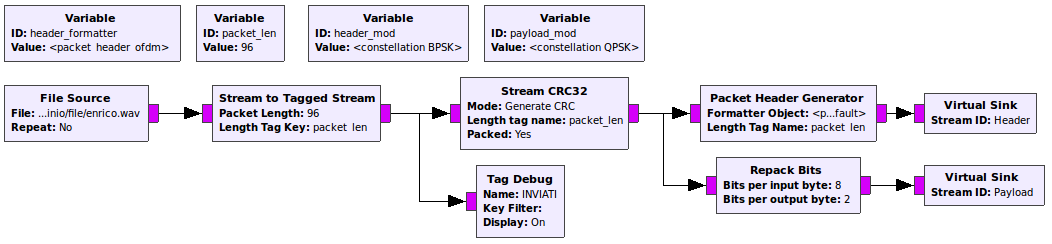
\includegraphics[scale=0.4]{Tx1}
 		\caption{}
 	\end{figure}
 Le informazioni vengono lette da file e fornite dal blocco "File Source" 8bit alla volta, questi campioni poi vengono aggregati 96 alla volta tramite l'aggiunta di un tag. A questo punto il blocco "CRC32" appende il codice di controllo per permettere al ricevitore di verificare la presenza di errori. I campioni a questo punto vengono processati sia dal blocco "Repack bits" che ha il compito di generare quattro nuovi byte con soli due bit dell'input (la costellazione qpsk permette l'invio di 2 bit alla volta quindi i 6 restanti lasciati a zero e verranno ignorati) che dal blocco "Packet Header generator". Quest'ultimo ha il compito di generare gli header dei pacchetti che permettono al ricevitore di riconoscere l'inizio di un blocco di 96byte di informazione. Gnuradio mette a disposizione degli oggetti "costellation" che contengono informazioni utili relative alle caratteristiche delle costellazioni, ad esempio il numero di bit significativi per la costellazione oppure la mappatura fra bit e punti delle costellazioni (Ad esempio l' oggetto digital.constellation\_qpsk viene utilizzato nel modulo "Repack bits" chiamando la funzione payload\_mod.bits\_per\_symbol() che restituisce 2). Le informazioni vengono poi trasferite a due "Virtual Sink" che fungono solamente da collegamento logico verso i "Virtual Source", il loro scopo è solamente quello di rendere la composizione più leggibile.
 	\item \subsection{Codifica informazioni in Simboli}
 	\begin{figure}[h]
 		\centering
 		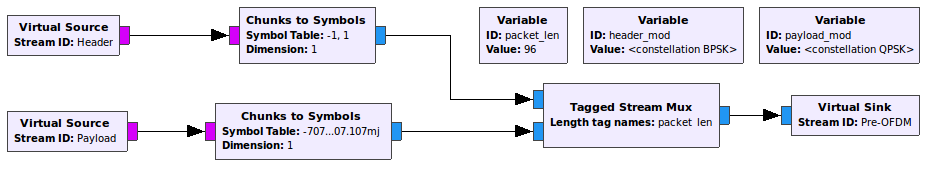
\includegraphics[scale=0.4]{Tx2}
 		\caption{}
 	\end{figure}
 Questa sezione del trasmettitore riceve due flussi dalla precedente contenenti i bit divisi fra header e payload. Il blocchi "Chunks to Symbols" convertono i bit (che ricordiamo sono già nel formato 1 bit significativo per byte per l' header e 2 bit significativi per byte per il payload) in numeri complessi della rispettiva costellazione. La mappatura fra bit significativi e numeri complessi viene fornita dall'oggetto di appoggio disponibile per le varie modulazioni fornito da gnuradio descritto brevemente nel punto precedente utilizzato chiamando rispettivamente le funzioni payload\_mod.points() e header\_mod.points(). A questo punto è necessario unire in un solo flusso (mantenendo la divisione fedele ai blocchi iniziali) i punti delle costellazioni ottenuti ricalcolando il tag della lunghezza, questo lavoro viene eseguito dal blocco "Tagged Stream Mux".
 	\item \subsection{Allocazione simboli sulle sottoportanti e creazione campioni per l'SDR}
 	\begin{figure}[h]
 		\centering
 		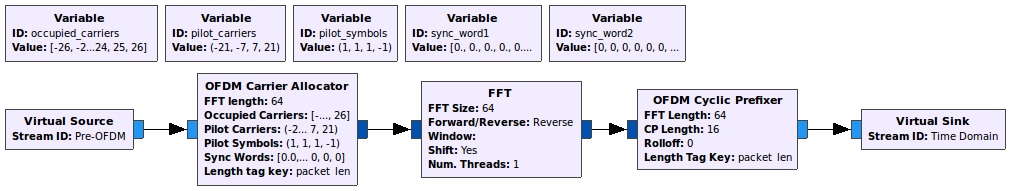
\includegraphics[scale=0.4]{Tx3}
 		\caption{}
 	\end{figure}
 L' obiettivo di questa sezione è quello di allocare sulle sottoportanti di OFDM le informazioni e creare i campioni da spedire nel dominio del tempo. Il blocco "OFDM Carrier Allocator" si occupa di allocare i punti delle costellazioni e i simboli pilota (pilot\_symbols) rispettivamente alle sottoportanti definite come occupied\_carriers e pilot\_carriers. Inoltre aggiunge all'inizio di ogni blocco trasmesso i sync\_words utilizzati dal ricevitore per sincronizzazione ed equalizzazione. L'output rappresenta un simbolo OFDM pronto per essere portato nel dominio del tempo dal blocco  "FFT" che esegue appunto la trasformata di fourier veloce. Il blocco "OFDM Cyclic Prefixer" aggiunge il prefisso ciclico spiegato in precedenza.
 
 	\item \subsection{Passaggio dati all'SDR}
 	\begin{figure}[h]
 		\centering
 		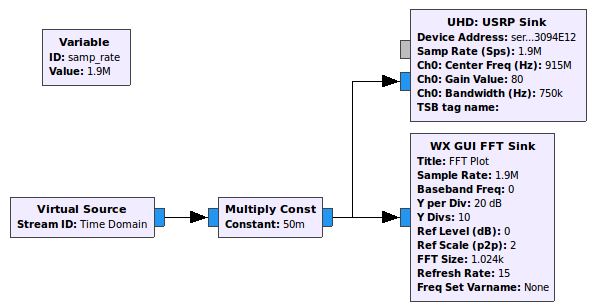
\includegraphics[scale=0.4]{Tx4}
 		\caption{}
 	\end{figure}
 \end{itemize}
L'ultima operazione consiste nel passare il simbolo OFDM al driver dell'SDR configurandolo con i parametri necessari per la trasmissione. Il blocco "WX GUI FFT Sink" serve per avere un feedback sulla trasmissione mostrando un grafico sul dominio delle frequenze.
 \section{Ricevitore}
 La ricezione è composta da tre sezioni principali connesse fra loro.
 \begin{itemize}
 	\item \subsection{Ricezione informazioni, sincronizzazione}
 	\begin{figure}[h]
 		\centering
 		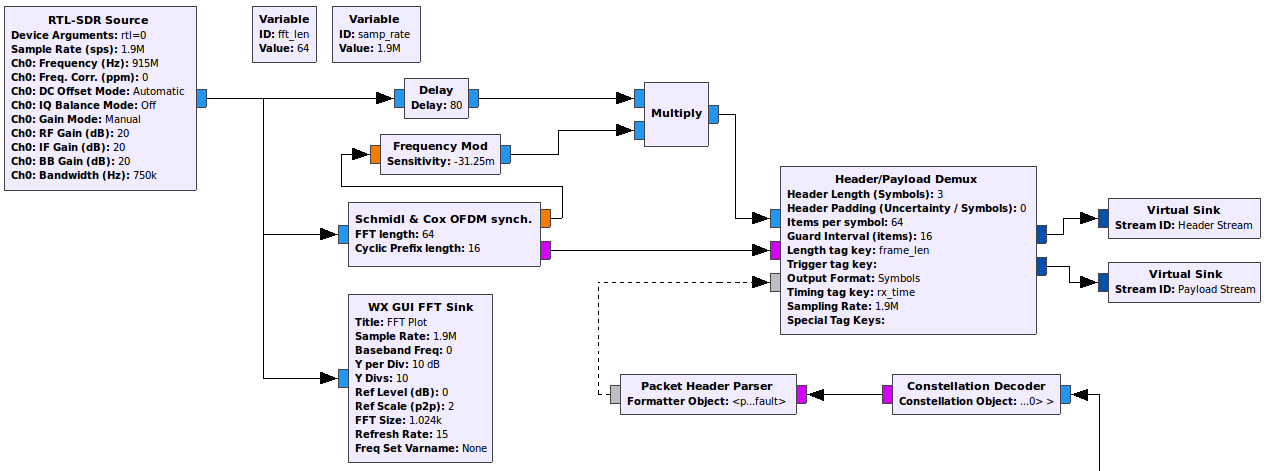
\includegraphics[scale=0.4]{Rx1}
 		\caption{}
 	\end{figure}
 Questa prima sezione del ricevitore ha il compito di leggere i campionamenti forniti dal driver per l'rtl-sdr e ottenere le informazioni nuovamente divise fra header e payload. Il blocco centrale di questa sezione è senzadubbio "Header/payload Demux" che ha il compito di dividere i campionamenti di header da quelli di payload per poi poter essere analizzati. I campionamenti sono forniti in forma complessa (I/Q) e rappresentano l'ampiezza in del segnale in quell'istante ma anche l' andamento della funzione che lo ha generato. 
 	\item \subsection{Equalizzazione e ottenimento simboli}
 	\begin{figure}[h]
 		\centering
 		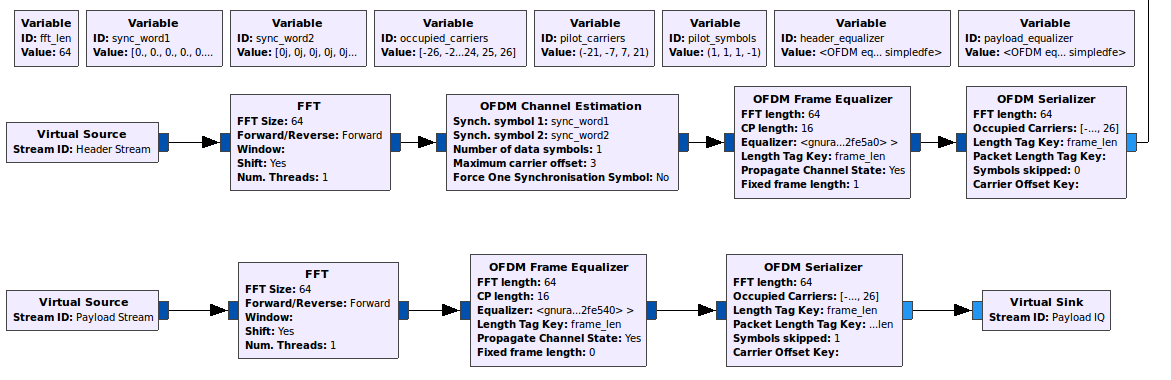
\includegraphics[scale=0.4]{Rx2}
 		\caption{}
 	\end{figure}
 	\item \subsection{Decodifica payload e scrittura file}
 	\begin{figure}[h]
 		\centering
 		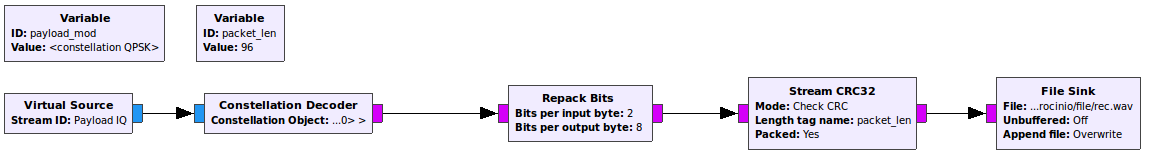
\includegraphics[scale=0.4]{Rx3}
 		\caption{}
 	\end{figure}
 \end{itemize}



